\section{作业及答案：结构力学基础与技巧班第7次作业及答案（三铰拱）}
\begin{analysisbox}
三铰拱利用中铰弯矩为零求水平推力，再用截面平衡求轴力、剪力和弯矩。注意拱轴线高度会直接影响弯矩表达式。
\end{analysisbox}
\subsection*{第 1 页转写}
五、练习题

2-40图2-188所示三铰拱截面K的弯矩为

（下拉为正），拱轴线方程为

4f

12

（la一 ）。（广西大学2010）

2-41

图2-189所示三铰拱的水平支座反力是多少？（武汉大学2010）

20kN/m

48kN

20kN

20kN

10m

6m

6m

6m

图2-188

图2-189

图2-190所示结构中，链杆AB的轴力为

2-42

。（以受拉为正）（中南大学

2010)

2-43图2-191所示三铰拱，拱轴线方程为y

(lz r )，其中f=4m，l=16m，

则截面D弯矩Mp等于

，截面D剪力FQD等于

。（浙江大学2012)

1/2

8m

图2-190

图2\textasciitilde{}191

六、练习题答案

2-40

13.33kN m。

2-41

45kN。

2-42

一Fp（压力）。

2-43

4q（上侧受拉）；0。
\begin{figure}[H]\centering
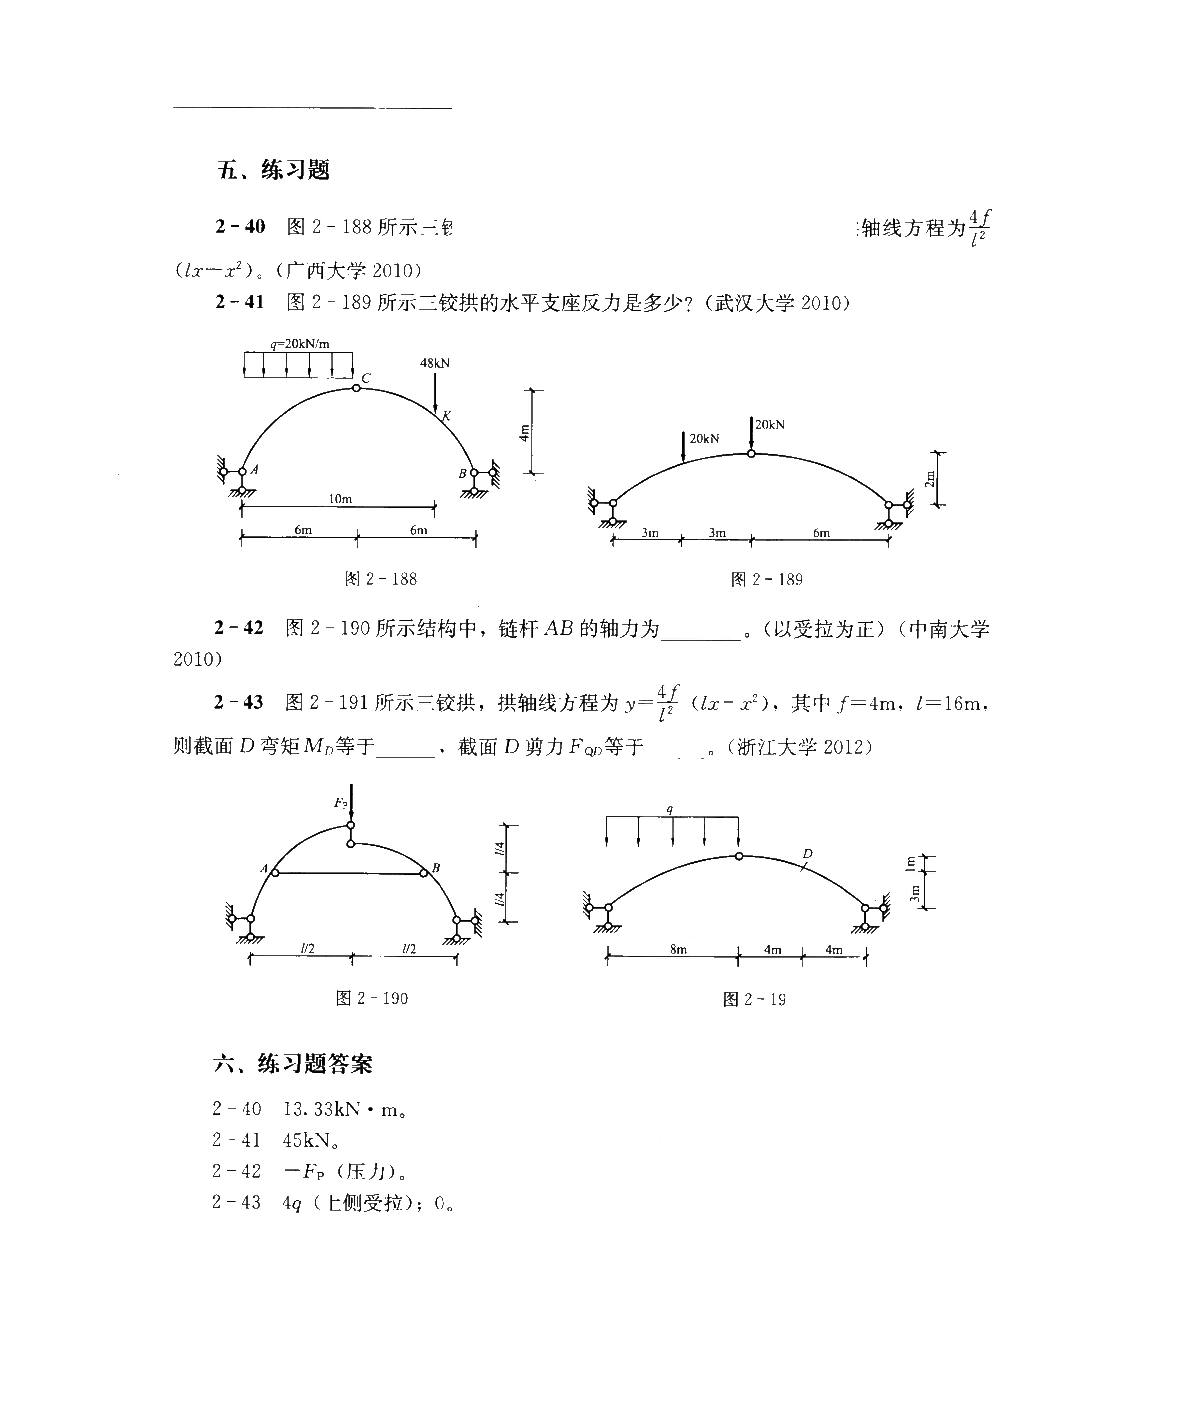
\includegraphics[width=0.92\textwidth]{figures/src10_p001.jpg}
\caption{结构力学基础与技巧班第7次作业及答案（三铰拱） 第 1 页清理图形页}
\end{figure}
